%%%%%%%%%%%%%%%%%%%%%%%%%%%%%%%%%%%%%%%%%%%%%%%%%%%%%%%%%%%%%%%%%%%%%%%%%%%%%%%
% CASE STUDY TEMPLATE - Programming and Problem Solving
% Author: Brendan Shea, PhD
% Course: Programming and Problem Solving
% Rochester Community and Technical College
%%%%%%%%%%%%%%%%%%%%%%%%%%%%%%%%%%%%%%%%%%%%%%%%%%%%%%%%%%%%%%%%%%%%%%%%%%%%%%%

\documentclass[11pt,letterpaper]{article}

%---------- PACKAGES ----------%
\usepackage[margin=1in, headheight=22pt]{geometry}
\usepackage[T1]{fontenc}
\usepackage{xcolor}
\usepackage{tcolorbox}
\usepackage{graphicx}
\usepackage{titlesec}
\usepackage{enumitem}
\usepackage{fancyhdr}
\usepackage{listings}
\usepackage{hyperref}
\usepackage{multicol}
\usepackage{booktabs}
\usepackage{tikz}
\usepackage{float}
\usepackage{amssymb}
\usepackage{amsmath}
\usepackage{pifont}

% TikZ libraries
\usetikzlibrary{shapes.geometric, arrows.meta, positioning, calc, backgrounds, fit, matrix, decorations.pathreplacing}

% Load tcolorbox libraries
\tcbuselibrary{skins,breakable,listings,listingsutf8}

%---------- COLOR DEFINITIONS ----------%
\definecolor{csprimary}{HTML}{2C3E50}
\definecolor{cssecondary}{HTML}{E74C3C}
\definecolor{cstertiary}{HTML}{3498DB}
\definecolor{csaccent}{HTML}{27AE60}
\definecolor{cswarm}{HTML}{F39C12}
\definecolor{cslight}{HTML}{ECF0F1}
\definecolor{csdark}{HTML}{1A252F}

% Syntax highlighting colors
\definecolor{codegreen}{HTML}{27AE60}
\definecolor{codepurple}{HTML}{9B59B6}
\definecolor{codeorange}{HTML}{E67E22}
\definecolor{codeblue}{HTML}{3498DB}
\definecolor{codegray}{HTML}{95A5A6}
\definecolor{codestring}{HTML}{E74C3C}
\definecolor{codebg}{HTML}{1E2A38}

%---------- CASE STUDY METADATA ----------%
\newcommand{\cstitle}{Never Trust the User}
\newcommand{\cssubtitle}{Secure Coding and Input Validation}
\newcommand{\csauthor}{Brendan Shea, PhD}
\newcommand{\cscourse}{Programming and Problem Solving}
\newcommand{\csinstitution}{Rochester Community and Technical College}
\newcommand{\csdate}{\today}

%---------- LISTINGS CONFIGURATION ----------%
\lstdefinestyle{basestyle}{
    backgroundcolor=\color{codebg},
    basicstyle=\ttfamily\small\color{white},
    breakatwhitespace=false,
    breaklines=true,
    captionpos=b,
    keepspaces=true,
    showspaces=false,
    showstringspaces=false,
    showtabs=false,
    tabsize=4,
    frame=none,
    xleftmargin=4mm,
    xrightmargin=4mm,
    aboveskip=0pt,
    belowskip=0pt,
}

\lstdefinestyle{javastyle}{
    style=basestyle,
    language=Java,
    keywordstyle=\color{codeblue}\bfseries,
    commentstyle=\color{codegray}\itshape,
    stringstyle=\color{codestring},
    morekeywords={String, Scanner, System, var, boolean, Math, Integer, throws},
}

\lstdefinestyle{cstyle}{
    style=basestyle,
    language=C,
    keywordstyle=\color{codeblue}\bfseries,
    commentstyle=\color{codegray}\itshape,
    stringstyle=\color{codestring},
}

\lstdefinestyle{sqlstyle}{
    style=basestyle,
    keywordstyle=\color{codeblue}\bfseries,
    morekeywords={SELECT, FROM, WHERE, DROP, TABLE, INSERT, DELETE, OR, AND},
}

%---------- CUSTOM ENVIRONMENTS ----------%
\newcommand{\keyterm}[1]{\textbf{\textcolor{cssecondary}{#1}}}

\newtcolorbox{conceptbox}[1][]{
    enhanced,
    colback=cslight,
    colframe=csprimary,
    fonttitle=\bfseries\color{white},
    title=#1,
    attach boxed title to top left={yshift=-2mm, xshift=5mm},
    boxed title style={colback=csprimary},
    breakable
}

\newtcolorbox{historybox}[1][]{
    enhanced,
    colback=codepurple!8,
    colframe=codepurple,
    fonttitle=\bfseries\color{white},
    title=#1,
    attach boxed title to top left={yshift=-2mm, xshift=5mm},
    boxed title style={colback=codepurple},
    breakable
}

\newtcolorbox{dangerbox}[1][]{
    enhanced,
    colback=cssecondary!8,
    colframe=cssecondary,
    fonttitle=\bfseries\color{white},
    title=#1,
    attach boxed title to top left={yshift=-2mm, xshift=5mm},
    boxed title style={colback=cssecondary},
    breakable
}

\newtcolorbox{safebox}[1][]{
    enhanced,
    colback=csaccent!8,
    colframe=csaccent,
    fonttitle=\bfseries\color{white},
    title=#1,
    attach boxed title to top left={yshift=-2mm, xshift=5mm},
    boxed title style={colback=csaccent},
    breakable
}

\newtcblisting{javacode}[1][]{
    enhanced,
    colback=codebg,
    colframe=csaccent,
    colupper=white,
    fonttitle=\bfseries\color{white},
    title=#1,
    attach boxed title to top left={yshift=-2mm, xshift=5mm},
    boxed title style={colback=csaccent},
    left=0mm, right=0mm, top=2mm, bottom=2mm,
    boxrule=1pt,
    breakable,
    pad at break=2mm,
    listing only,
    listing options={style=javastyle}
}

\newtcblisting{ccode}[1][]{
    enhanced,
    colback=codebg,
    colframe=cssecondary,
    colupper=white,
    fonttitle=\bfseries\color{white},
    title=#1,
    attach boxed title to top left={yshift=-2mm, xshift=5mm},
    boxed title style={colback=cssecondary},
    left=0mm, right=0mm, top=2mm, bottom=2mm,
    boxrule=1pt,
    breakable,
    pad at break=2mm,
    listing only,
    listing options={style=cstyle}
}

\newtcblisting{sqlcode}[1][]{
    enhanced,
    colback=codebg,
    colframe=cswarm,
    colupper=white,
    fonttitle=\bfseries\color{white},
    title=#1,
    attach boxed title to top left={yshift=-2mm, xshift=5mm},
    boxed title style={colback=cswarm},
    left=0mm, right=0mm, top=2mm, bottom=2mm,
    boxrule=1pt,
    breakable,
    pad at break=2mm,
    listing only,
    listing options={style=sqlstyle}
}

\newtcolorbox{questionbox}{
    enhanced,
    colback=cswarm!10,
    colframe=cswarm,
    fonttitle=\bfseries\color{white},
    title=Discussion Questions,
    attach boxed title to top center={yshift=-2mm},
    boxed title style={colback=cswarm},
    breakable
}

\newtcolorbox{glossarybox}{
    enhanced,
    colback=cslight,
    colframe=csprimary,
    fonttitle=\bfseries\color{white},
    title=Glossary of Key Terms,
    attach boxed title to top center={yshift=-2mm},
    boxed title style={colback=csprimary},
    breakable
}

%---------- HEADER/FOOTER ----------%
\pagestyle{fancy}
\fancyhf{}
\fancyhead[L]{\small\textcolor{csprimary}{\cscourse}}
\fancyhead[R]{\small\textcolor{csprimary}{Case Study}}
\fancyfoot[C]{\thepage}
\renewcommand{\headrulewidth}{0.4pt}
\renewcommand{\headrule}{\hbox to\headwidth{\color{csprimary}\leaders\hrule height \headrulewidth\hfill}}

%---------- SECTION FORMATTING ----------%
\titleformat{\section}
    {\Large\bfseries\color{csprimary}}
    {\thesection}{1em}{}[\color{cssecondary}\titlerule]
    
\titleformat{\subsection}
    {\large\bfseries\color{cstertiary}}
    {\thesubsection}{1em}{}

%---------- HYPERLINK SETTINGS ----------%
\hypersetup{
    colorlinks=true,
    linkcolor=cstertiary,
    urlcolor=cstertiary
}

%%%%%%%%%%%%%%%%%%%%%%%%%%%%%%%%%%%%%%%%%%%%%%%%%%%%%%%%%%%%%%%%%%%%%%%%%%%%%%%
\begin{document}

%---------- TITLE BLOCK ----------%
\begin{tcolorbox}[
    enhanced,
    colback=csprimary,
    colframe=csprimary,
    arc=0mm,
    left=10mm, right=10mm, top=8mm, bottom=8mm
]
\begin{center}
    {\huge\bfseries\color{white}\cstitle}\\[3mm]
    {\Large\color{cslight}\cssubtitle}\\[5mm]
    \textcolor{cssecondary}{\rule{0.5\textwidth}{1pt}}\\[5mm]
    {\large\color{white}\csauthor}\\[2mm]
    {\normalsize\color{cslight}\cscourse\ $\bullet$ \csinstitution}
\end{center}
\end{tcolorbox}

\vspace{5mm}

%---------- INTRODUCTION ----------%
\section*{Introduction}

In 1988, a graduate student named Robert Morris released a program that brought roughly 10\% of the entire Internet to its knees. The \keyterm{Morris Worm} exploited several vulnerabilities, including a classic input validation flaw: a program that copied user input into memory without checking how much data it received. Morris's ``experiment'' caused millions of dollars in damage and earned him the first conviction under the Computer Fraud and Abuse Act.

The lesson from 1988 remains the cardinal rule of secure programming: \textbf{Never trust the user.} Every piece of data entering your program---from keyboard input to file uploads to network messages---is potentially malicious. Attackers have spent decades crafting inputs designed to make programs behave in unintended ways, and they've succeeded spectacularly: data breaches, stolen passwords, crashed systems, and compromised infrastructure.

This case study explores the art of \keyterm{input validation}---checking that data meets your expectations before using it. You'll learn why validation matters, how attackers exploit its absence, and how to write code that defends itself.

\begin{conceptbox}[The Fundamental Principle]
\textbf{All input is guilty until proven innocent.} Whether it comes from a user typing at a keyboard, a file on disk, a network connection, or another program, you must validate data before trusting it. The consequences of failing to do so range from crashed programs to catastrophic security breaches.
\end{conceptbox}

%---------- A BRIEF HISTORY ----------%
\section{A Brief History of Things Going Wrong}

Understanding security requires understanding how attackers think. Let's examine some landmark incidents that shaped our understanding of input validation.

\begin{historybox}[The Morris Worm (1988)]
Robert Morris, a Cornell graduate student and son of a chief scientist at the NSA, released a self-replicating program intended to gauge the size of the Internet. It exploited buffer overflows in the \texttt{fingerd} and \texttt{sendmail} programs---services that blindly copied user input without checking its length. The worm spread faster than anticipated, reinfecting machines and consuming resources until systems ground to a halt. Morris was fined \$10,050, sentenced to probation, and required to perform community service. He later became a professor at MIT. The incident led to the creation of CERT (Computer Emergency Response Team), the first organization dedicated to coordinating responses to security incidents.
\end{historybox}

\begin{historybox}[SQL Injection Attacks (2000s--Present)]
In 2008, a SQL injection attack compromised Heartland Payment Systems, exposing 130 million credit card numbers---the largest data breach in history at that time. The attacker inserted malicious database commands through a web form that failed to validate its input. SQL injection remains in the OWASP Top 10 security vulnerabilities decades after it was first documented, because developers keep making the same mistake: constructing database queries by concatenating user input.
\end{historybox}

\begin{historybox}[The Equifax Breach (2017)]
Attackers exploited a vulnerability in Apache Struts, a web application framework, to breach Equifax. The flaw allowed attackers to execute arbitrary code through maliciously crafted input. The breach exposed personal information of 147 million people---Social Security numbers, birth dates, addresses, and driver's license numbers. Equifax had failed to patch a known vulnerability for months, but the underlying issue was the same: insufficient input validation in the framework's code.
\end{historybox}

\begin{historybox}[Log4Shell (2021)]
A vulnerability in Log4j, a ubiquitous Java logging library, allowed attackers to execute code simply by sending specially crafted text strings. If a vulnerable application logged user input (like a username or search query), the attacker's payload would execute. The vulnerability, called Log4Shell, affected millions of applications worldwide---from Minecraft servers to Apple's iCloud. It demonstrated that even ``safe'' operations like logging can be dangerous if input isn't properly sanitized.
\end{historybox}

These incidents share a common thread: programs that accepted data without adequate scrutiny. The specific mechanisms differ, but the fundamental failure is the same.

%---------- WHY JAVA IS SAFER ----------%
\section{Why Java Is Safer (But Not Safe)}

Java was designed in the 1990s with security in mind, learning from decades of vulnerabilities in C and C++. Several language features provide protection that C programmers must implement manually---or more often, forget to implement.

\subsection{Memory Safety and Bounds Checking}

In C, arrays are just pointers to memory. Nothing stops you from reading or writing past the end of an array:

\begin{ccode}[C: No Bounds Checking (Dangerous!)]
char buffer[10];
// C allows this -- writes past the end of the array!
strcpy(buffer, "This string is way too long for the buffer");
// Memory corruption: other variables, return addresses overwritten
\end{ccode}

This is a \keyterm{buffer overflow}---the foundation of countless exploits including the Morris Worm. Attackers craft input that overflows a buffer and overwrites critical data structures, potentially gaining control of the program.

Java prevents this entirely:

\begin{javacode}[Java: Automatic Bounds Checking]
int[] array = new int[10];
array[15] = 42;  // Throws ArrayIndexOutOfBoundsException
// Program crashes safely rather than corrupting memory
\end{javacode}

Every array access in Java is checked at runtime. If you try to access an invalid index, Java throws an exception rather than corrupting memory. This single feature eliminates an entire class of vulnerabilities.

\begin{center}
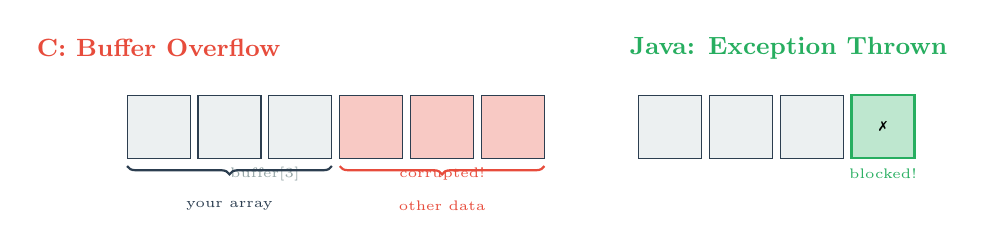
\begin{tikzpicture}[
    mem/.style={rectangle, draw=csprimary, minimum width=8mm, minimum height=8mm, font=\tiny\ttfamily},
    arrow/.style={-{Stealth[length=2mm]}, thick}
]

% C memory model
\node[font=\small\bfseries, color=cssecondary] at (0,1.5) {C: Buffer Overflow};

\foreach \i/\c in {0/cslight, 1/cslight, 2/cslight, 3/cssecondary!30, 4/cssecondary!30, 5/cssecondary!30} {
    \node[mem, fill=\c] at (\i*0.9,0.5) {};
}
\node[font=\tiny, color=codegray] at (1.35,-0.1) {buffer[3]};
\node[font=\tiny, color=cssecondary] at (3.6,-0.1) {corrupted!};

\draw[decorate, decoration={brace, amplitude=3pt, mirror}, thick, csprimary] 
    (-0.4,0) -- (2.2,0);
\node[font=\tiny, color=csprimary] at (0.9,-0.5) {your array};

\draw[decorate, decoration={brace, amplitude=3pt, mirror}, thick, cssecondary] 
    (2.3,0) -- (4.9,0);
\node[font=\tiny, color=cssecondary] at (3.6,-0.5) {other data};

% Java memory model  
\node[font=\small\bfseries, color=csaccent] at (8,1.5) {Java: Exception Thrown};

\foreach \i in {0,1,2} {
    \node[mem, fill=cslight] at (6.5+\i*0.9,0.5) {};
}
\node[mem, fill=csaccent!30, draw=csaccent, thick] at (9.2,0.5) {\ding{55}};

\node[font=\tiny, color=csaccent] at (9.2,-0.1) {blocked!};

\end{tikzpicture}
\end{center}

\subsection{No Pointer Arithmetic}

In C, you can manipulate memory addresses directly, pointing to arbitrary locations. Java has references but no pointer arithmetic---you cannot calculate memory addresses or access memory that wasn't properly allocated.

\subsection{Automatic Memory Management}

C requires programmers to manually allocate and free memory. Mistakes lead to ``use-after-free'' vulnerabilities---accessing memory that's been returned to the system and might now contain attacker-controlled data. Java's garbage collector handles memory automatically, eliminating this class of bugs.

\subsection{The Catch: Logic Bugs Remain}

Java's safety features prevent low-level memory corruption, but they cannot prevent logic errors. If your code trusts user input when it shouldn't, Java won't save you:

\begin{javacode}[Java: Still Vulnerable to Logic Bugs]
// User provides their "age"
String input = scanner.nextLine();
int age = Integer.parseInt(input);  

// What if input is "-5"? "999"? "0"?
// Java won't stop you from using an invalid age
if (age >= 18) {
    grantAccess();  // Attacker enters "999", bypasses check
}
\end{javacode}

This is where input validation comes in.

%---------- TYPES OF ATTACKS ----------%
\section{Types of Input-Based Attacks}

Attackers have developed numerous techniques for exploiting insufficient input validation. Understanding these attacks helps you defend against them.

\subsection{SQL Injection}

\keyterm{SQL injection} occurs when user input is incorporated directly into database queries. Imagine a login form:

\begin{javacode}[Vulnerable: String Concatenation in SQL]
String username = scanner.nextLine();
String password = scanner.nextLine();

// DANGEROUS: Building query with user input
String query = "SELECT * FROM users WHERE name='" + username 
             + "' AND password='" + password + "'";
\end{javacode}

If a user enters the username \texttt{admin' --}, the query becomes:

\begin{sqlcode}[The Resulting Query]
SELECT * FROM users WHERE name='admin' --' AND password=''
\end{sqlcode}

The \texttt{--} is a SQL comment, so everything after it is ignored. The attacker logs in as admin without knowing the password! Even worse, an attacker could enter \texttt{'; DROP TABLE users; --} and delete your entire user database.

\begin{safebox}[Defense: Parameterized Queries]
Never build SQL queries by concatenating strings. Use parameterized queries (prepared statements) that separate code from data:
\begin{center}
\texttt{PreparedStatement ps = conn.prepareStatement(}\\
\texttt{~~~~"SELECT * FROM users WHERE name=? AND password=?");}\\
\texttt{ps.setString(1, username);}\\
\texttt{ps.setString(2, password);}
\end{center}
The database treats parameters as pure data, never as SQL commands.
\end{safebox}

\subsection{Command Injection}

Similar to SQL injection, \keyterm{command injection} occurs when user input is passed to system commands:

\begin{javacode}[Vulnerable: Command Injection]
String filename = scanner.nextLine();
// DANGEROUS: User input in system command
Runtime.getRuntime().exec("ls " + filename);

// Attacker enters: "file.txt; rm -rf /"
// Command becomes: ls file.txt; rm -rf /
// Second command deletes everything!
\end{javacode}

\subsection{Cross-Site Scripting (XSS)}

In web applications, \keyterm{cross-site scripting} occurs when user input is displayed on a page without escaping. An attacker might enter their ``name'' as:

\texttt{<script>stealCookies()</script>}

If the website displays this without sanitization, the script executes in other users' browsers, potentially stealing their session cookies or credentials.

\subsection{Integer Overflow}

Even numeric input can be dangerous. What happens when arithmetic exceeds the maximum value a type can hold?

\begin{javacode}[Integer Overflow]
int quantity = scanner.nextInt();  // User enters 2,000,000,000
int price = 10;
int total = quantity * price;      // Overflow! Result is negative

if (total > 0) {
    chargeCustomer(total);  // Doesn't execute -- total is negative!
}
// Attacker gets items for free (or gets paid!)
\end{javacode}

%---------- VALIDATION IN PRACTICE ----------%
\section{Input Validation in Practice}

Now let's see how to validate input properly. The goal is to reject bad data before it can cause harm.

\subsection{Validating Numeric Input}

The \texttt{Scanner} class can throw exceptions if users enter non-numeric data when you expect numbers:

\begin{javacode}[Handling Non-Numeric Input]
Scanner scanner = new Scanner(System.in);
System.out.print("Enter your age: ");

int age;
if (scanner.hasNextInt()) {
    age = scanner.nextInt();
} else {
    System.out.println("Error: Please enter a number.");
    scanner.next();  // Clear the invalid input
    return;
}
\end{javacode}

But that's only half the battle---you must also check that the number is \textit{reasonable}:

\begin{javacode}[Complete Numeric Validation]
public static int getValidAge(Scanner scanner) {
    while (true) {
        System.out.print("Enter your age: ");
        
        // Check 1: Is it an integer?
        if (!scanner.hasNextInt()) {
            System.out.println("Please enter a whole number.");
            scanner.next();  // discard invalid input
            continue;
        }
        
        int age = scanner.nextInt();
        
        // Check 2: Is it in a valid range?
        if (age < 0) {
            System.out.println("Age cannot be negative.");
            continue;
        }
        if (age > 150) {
            System.out.println("Please enter a realistic age.");
            continue;
        }
        
        return age;  // Passed all checks!
    }
}
\end{javacode}

\subsection{Validating String Input}

String validation depends on what the string represents. For a username, you might check:

\begin{javacode}[String Validation Example]
public static boolean isValidUsername(String username) {
    // Check 1: Not null or empty
    if (username == null || username.isEmpty()) {
        return false;
    }
    
    // Check 2: Length constraints
    if (username.length() < 3 || username.length() > 20) {
        return false;
    }
    
    // Check 3: Only allowed characters (letters, numbers, underscore)
    if (!username.matches("^[a-zA-Z0-9_]+$")) {
        return false;
    }
    
    // Check 4: Doesn't start with a number
    if (Character.isDigit(username.charAt(0))) {
        return false;
    }
    
    return true;
}
\end{javacode}

\subsection{The Whitelist Approach}

There are two philosophies for validation:
\begin{itemize}[itemsep=2pt]
    \item \textbf{Blacklist}: Block known bad inputs (dangerous characters, malicious patterns)
    \item \textbf{Whitelist}: Allow only known good inputs (specific characters, formats, ranges)
\end{itemize}

\keyterm{Whitelisting} is almost always safer. Blacklists are fragile---attackers constantly find new ways to encode malicious input that bypasses filters. With whitelisting, anything you haven't explicitly approved is rejected.

\begin{center}
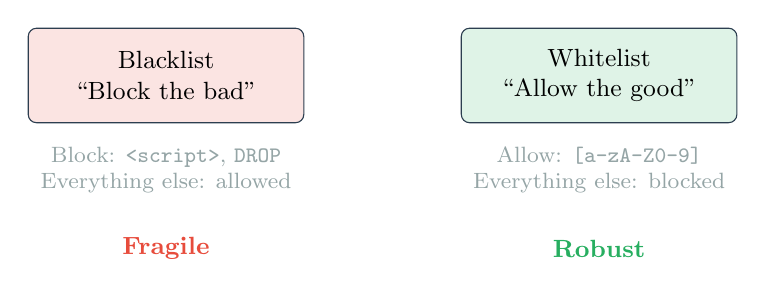
\begin{tikzpicture}[
    box/.style={rectangle, rounded corners=3pt, draw=csprimary, fill=#1, minimum width=35mm, minimum height=12mm, font=\small, align=center},
    arrow/.style={-{Stealth[length=2mm]}, thick}
]

% Blacklist
\node[box=cssecondary!15] (black) at (0,0) {Blacklist\\``Block the bad''};
\node[font=\footnotesize, color=codegray, align=center] at (0,-1.2) {Block: \texttt{<script>}, \texttt{DROP}\\Everything else: allowed};

% Whitelist
\node[box=csaccent!15] (white) at (5.5,0) {Whitelist\\``Allow the good''};
\node[font=\footnotesize, color=codegray, align=center] at (5.5,-1.2) {Allow: \texttt{[a-zA-Z0-9]}\\Everything else: blocked};

% Verdict
\node[font=\small\bfseries, color=cssecondary] at (0,-2.2) {Fragile};
\node[font=\small\bfseries, color=csaccent] at (5.5,-2.2) {Robust};

\end{tikzpicture}
\end{center}

%---------- DEFENSE IN DEPTH ----------%
\section{Defense in Depth}

No single validation check is foolproof. Security experts advocate \keyterm{defense in depth}---multiple layers of protection so that if one fails, others still provide security.

\begin{center}
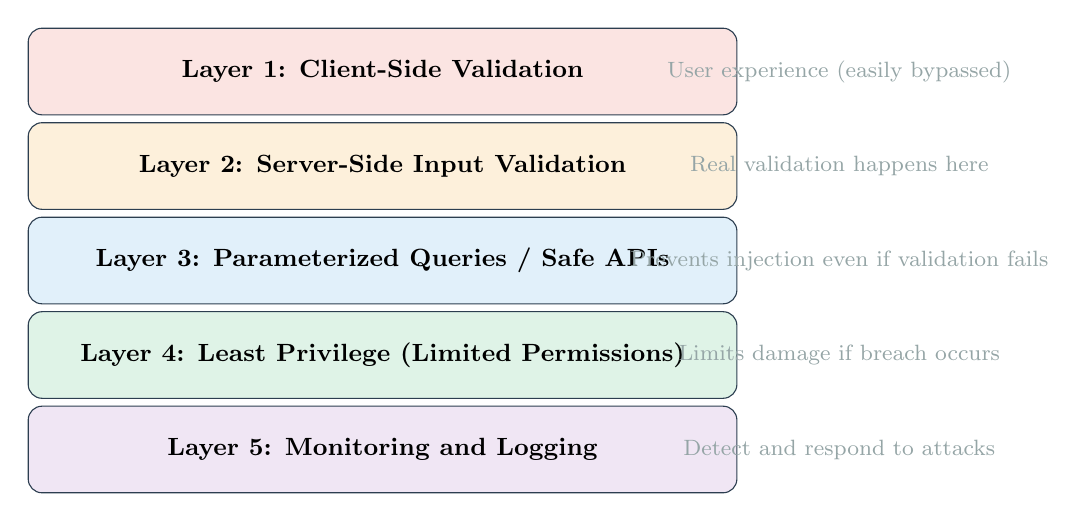
\begin{tikzpicture}[
    layer/.style={rectangle, rounded corners=5pt, draw=csprimary, fill=#1, minimum width=90mm, minimum height=11mm, font=\small\bfseries},
]

\node[layer=cssecondary!15] (l1) at (0,2.4) {Layer 1: Client-Side Validation};
\node[layer=cswarm!15] (l2) at (0,1.2) {Layer 2: Server-Side Input Validation};
\node[layer=cstertiary!15] (l3) at (0,0) {Layer 3: Parameterized Queries / Safe APIs};
\node[layer=csaccent!15] (l4) at (0,-1.2) {Layer 4: Least Privilege (Limited Permissions)};
\node[layer=codepurple!15] (l5) at (0,-2.4) {Layer 5: Monitoring and Logging};

\node[font=\footnotesize\color{codegray}] at (5.8,2.4) {User experience (easily bypassed)};
\node[font=\footnotesize\color{codegray}] at (5.8,1.2) {Real validation happens here};
\node[font=\footnotesize\color{codegray}] at (5.8,0) {Prevents injection even if validation fails};
\node[font=\footnotesize\color{codegray}] at (5.8,-1.2) {Limits damage if breach occurs};
\node[font=\footnotesize\color{codegray}] at (5.8,-2.4) {Detect and respond to attacks};

\end{tikzpicture}
\end{center}

Client-side validation (in the browser, before data is sent) improves user experience but provides \textit{no security}---attackers can bypass it trivially. Real validation must happen on the server, where you control the code.

\subsection{Fail Securely}

When validation fails, your program must respond appropriately:

\begin{javacode}[Failing Securely]
public static void processOrder(String productId, int quantity) {
    // Validate product ID
    if (!isValidProductId(productId)) {
        // Log the attempt (for security monitoring)
        logger.warn("Invalid product ID attempted: " + sanitize(productId));
        // Return generic error (don't reveal what went wrong)
        throw new InvalidInputException("Invalid request");
    }
    
    // Validate quantity
    if (quantity < 1 || quantity > MAX_ORDER_QUANTITY) {
        logger.warn("Invalid quantity attempted: " + quantity);
        throw new InvalidInputException("Invalid request");
    }
    
    // Only proceed if ALL validation passes
    executeOrder(productId, quantity);
}
\end{javacode}

Notice several security practices: logging suspicious input for later analysis, returning generic error messages (detailed errors help attackers understand your validation), and processing only after \textit{all} checks pass.

%---------- PRINCIPLES ----------%
\section{Principles of Secure Input Handling}

Let's summarize the key principles:

\textbf{1. Validate all input.} Every piece of data from outside your program---user input, files, network data, environment variables, command-line arguments---must be validated.

\textbf{2. Validate on the server.} Client-side checks are for user convenience only. An attacker controls the client and can send anything.

\textbf{3. Use whitelists.} Define what's allowed rather than trying to enumerate everything that's forbidden.

\textbf{4. Validate type, length, format, and range.} Is it the right data type? Is it within acceptable length limits? Does it match the expected format? Is the value in a sensible range?

\textbf{5. Reject, don't sanitize.} It's tempting to ``fix'' bad input by removing dangerous characters. This is risky---attackers find creative encodings that bypass sanitization. When possible, reject invalid input entirely.

\textbf{6. Use safe APIs.} Parameterized SQL queries, safe HTML encoding functions, and well-tested libraries handle dangerous operations correctly. Don't reinvent the wheel.

\textbf{7. Apply least privilege.} Even if an attacker bypasses validation, limit the damage by running with minimal permissions. A web application shouldn't have database admin rights.

\textbf{8. Log and monitor.} Track validation failures. Patterns of invalid input often indicate attack attempts. You can't respond to attacks you don't know about.

The cost of implementing these practices is small compared to the cost of a breach. Security isn't a feature you add at the end---it's a mindset you apply from the first line of code.

%---------- DISCUSSION QUESTIONS ----------%
\section*{Discussion Questions}

\begin{questionbox}
\begin{enumerate}[leftmargin=*, label=\textcolor{cswarm}{\textbf{\arabic*.}}]
    \item \textbf{The Morris Worm Legacy:} Robert Morris exploited vulnerabilities in 1988, was convicted, and later became an MIT professor and successful entrepreneur. Some view him as a cautionary tale; others as a pioneer who exposed critical weaknesses. How should society treat security researchers who expose vulnerabilities through exploits? Is there a difference between malicious hacking and ``research''?

    \item \textbf{Language Design Trade-offs:} Java's bounds checking prevents buffer overflows but adds runtime overhead---every array access requires a check. C is faster but puts the burden on programmers. Is this trade-off worth it? Are there applications where C's approach is justified despite the risks?

    \item \textbf{The Equifax Question:} Equifax had months to patch a known vulnerability but failed to do so. Who bears responsibility: the programmers who wrote the vulnerable code, the managers who didn't prioritize patching, the executives, or the company as a whole? How should liability for security breaches be assigned?

    \item \textbf{Usability vs.\ Security:} Strict input validation can frustrate users. A name field that rejects ``O'Brien'' or ``José'' because of apostrophes and accents is both annoying and exclusionary. How do you balance security with usability and inclusion? What's the right approach for names, addresses, and other personal information?

    \item \textbf{The Arms Race:} Attackers constantly develop new techniques; defenders patch and add validation; attackers find bypasses. Is this cycle inevitable? Could programming languages, frameworks, or development practices fundamentally change this dynamic, or will security always be a cat-and-mouse game?
\end{enumerate}
\end{questionbox}

%---------- GLOSSARY ----------%
\section*{Key Terms}

\begin{glossarybox}
\begin{description}[leftmargin=!, labelwidth=3.4cm, font=\bfseries\color{cssecondary}]
    \item[Buffer Overflow] A vulnerability where input exceeds allocated memory, overwriting adjacent data and potentially allowing code execution.
    
    \item[Bounds Checking] Verifying that array accesses are within valid indices; Java does this automatically, C does not.
    
    \item[Command Injection] An attack where malicious input is executed as system commands due to improper validation.
    
    \item[Cross-Site Scripting] A web vulnerability where attacker-supplied scripts execute in victims' browsers.
    
    \item[Defense in Depth] A security strategy using multiple protective layers so that failure of one doesn't compromise the system.
    
    \item[Input Validation] The process of verifying that data meets expected criteria before processing it.
    
    \item[Integer Overflow] When arithmetic exceeds a type's maximum value and wraps around, potentially causing logic errors.
    
    \item[Morris Worm] The 1988 self-replicating program that exploited buffer overflows and brought down much of the Internet.
    
    \item[Parameterized Query] A database query where user input is passed as parameters rather than concatenated into the query string.
    
    \item[SQL Injection] An attack where malicious SQL commands are inserted through improperly validated input fields.
    
    \item[Sanitization] Modifying input to remove or escape dangerous characters---generally less safe than rejection.
    
    \item[Whitelisting] Validating by defining allowed inputs; anything not explicitly permitted is rejected.
\end{description}
\end{glossarybox}

\vspace{5mm}

%---------- FOOTER ----------%
\begin{center}
\textcolor{csprimary}{\rule{0.6\textwidth}{0.5pt}}\\[3mm]
{\small\textcolor{gray}{This case study is part of the Open Educational Resources for \cscourse.\\
Licensed under Creative Commons Attribution 4.0 (CC BY 4.0).}}
\end{center}

\end{document}